% -*- coding: UTF -*-
% Держать в начале каждого файла!

\documentclass[russian, 12pt]{article}
\usepackage{metod}

\MTDSetPhysSection{Механика}
\MTDSetTitle{Закручивание гаек осциллографами}
\MTDDesignator{М228}
\MTDSetGrade{13}

\MTDSetAuthors{И.~Н.~Грачева, В.~И.~Гребенкин, А.~Е.~Иванов, И.~А.~Коротова,
Е.~И.~Красавина, А.~В.~Кравцов, Н.~С.~Кулеба, Б.~В.~Падалкин,
Г.~Ю.~Шевцова, Т.~С.~Цвецинская}

\MTDSetEditorsGenCase{А. В. Кравцова и И. Н. Грачевой}


\begin{document}


\MTDTitlePage
\MTDInfoPage

\section{Гыгыгы}
\subsection{Лол}
\subsubsection{Варнинг C2231: Отвертка}
\MTDWarn{Осциллограф --- не отвертка. Не откручивать винты осциллографом! В рамках данной лабы --- только гайки! Откручивать винты осциллографом могут только в ПТУ, а здесь СУНЦ МГТУ им. Баумана! Думайте!}

Во-первых, перед ней выступал крайне скудный докладчик. Есть такая форма работы на Шаг в будущее, называется, "тупой абитуриент и НИИ": при этой форме работу (как правило, нечто годное) делает профессиональный инженер или даже коллектив, а тупой, собственно, абитуриент зачитывает наизусть доклад (в самом плохом случае доклад написан профессиональным пиарщиком из НИИ, был и такой абитуриент) и поступает, если не произойдёт страшного завала на вопросах из аудитории, хотя, как правило, к типичным вопросам ответы готовят заранее (или, теоретически, согласовывают с кем-то на кафедре, но мне точный характер этой коррупции не известен, кроме того, что какая-то коррупция есть точно). "НИИ" - не обязательно настоящий НИИ: Фенька, например, в качестве НИИ имела дедушку, который 93,34535\% работы и сделал (и теперь поступил, надо понимать, а она за него учится, старого лентяя).

\begin{table}[h!]
\caption{\indent Таблица с сфабрикованными данными}
\vspace{-0.25cm}
\begin{center}
\begin{tabular}{|p{1cm}|p{1cm}|p{1cm}|p{1cm}|p{1cm}|p{1cm}|p{1cm}|p{1cm}|p{1cm}|p{1cm}|}
\hline
$N$ & 1 & 2 & 3 & 4  & 5 & 6 & 7 & 8 & 9    \\
\hline
$l,\ \text{м}$ & 9,4 & 18,8 & 28,2 & 37,6 & 47,0 & 56,4 & 65,8 & 75,2 & 84,6   \\
\hline
$\Delta,\ \text{см}$ & 15 & 15 & 43 & 19 & 16 & 50 & 53 & 15 & 67   \\
\hline
\end{tabular}
\end{center}
\end{table}


\subsection{Довольно красивая девочка}
\subsubsection{Очень длинное предложение}



...Гайана Оттаровна оказалась довольно красивой девочкой. Стройная (но не слишком, без "ЭМ ЭС Эскцессов"); среднего роста (скажем, средний между моим и твоим); спокойных пропорций (пояснение к сему эпитету я придумал такое, осторожно, мелкое хамство: она красивая не оттого же, отчего красивой считается, скажем, пресловутый секс-символ ГБОУ лицея №1580 при МГТУ им. Н. Э. Баумана Нам-Всем-Известно-Что-За-Девочка-Особенно-Пономаренко-Известно-Да); улыбчивая (про это еще будут комментарии позже, ибо там всё не так просто); с лицом вполне красивым (особенно с некоторых ракурсов), но и достаточно "забавным" и несложным, чтобы не производить "модельного" (или гламурного, или вообще - идиотское прилагательное инбаунд, тэйк кавэр - шехерезадного) впечатления; то ли вообще без косметики, то ли крайне умеренно с, не разобрал точно; обладательница сравнительно (с некоторыми) коротких довольно смешных волос цвета буйной меди, убранных в пучок за головой, которые забавно смотрелись на фоне белого вязаного свитера и чёрных неформальных брюк-полуджинс, как ты часто (всегда? :) носишь.


\begin{figure}[h!]
\begin{center}
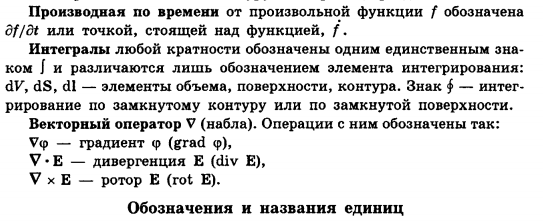
\includegraphics[keepaspectratio=true]{sample_fig}
\end{center}
\label{img:tank-wheel-mode}
\caption{\emph{Какая-то трепотня\label{img:tank-wheel-mode}}}
\end{figure}

\newpage

\paragraph{Дифференциальное уравнение колебаний.} На рассматриваемое тело
действуют следующие силы:
\begin{itemize}
  \item Сила тяжести $m\vec g$, направленная вниз.
  \item Сила сопротивления движению $-r \vec v$, направленная против
      вектора скорости $\vec v$.
  \item Силы упругости со стороны пружин, $ - k_1 \Delta l_1 = k_1 (x -
      l_{10}$ и $ - k_2 \Delta l_2 = k_2 (x - l_{20})$, где $x$ ---
      координата точки крепления пружин к телу (далее будем называть её
      просто координатой тела), $\Delta l_1$ и $\Delta l_2$ --- удлинения
      первой и второй пружин соответственно. Силы упругости направлены
      вверх, если пружины растянуты, и вниз, если пружины сжаты.
\end{itemize}
\section{А жареных гвоздей... Жареных гвоздей не хочешь?}
Запишем суммарную силу $R$, действующую на тело:
\[
 R = - k_1 (x - l_{10}) - k_2 (x - l_{20}) + m g - r  v.
\]
Учитывая, что $\vec v = \vec[.]x$, получим
\[
 R = - k_1 (x - l_{10}) - k_2 (x - l_{20}) + m g - r \dot x.
\]

Не заметил, что на ногах было, но надо предположить, что какие-то черные, не бликующие туфли без каблука типа тех, что скаутше я надел, или же в целом аналогичные ботинки (белый цвет, блики и каблук я бы точно заметил, а раз не заметил, значит было именно что-то такое, потому что в этом смысле я не отличаюсь от котов: блики привлекают внимание!).

фжлыдвоалджыоадлфвоыад рфав олвфыло афлыва
\end{document}

